\documentclass[a4paper,11pt]{article}
\usepackage[francais]{babel}
%% Prévu pour compiler avec lualatex
% \usepackage[utf8]{inputenc}
\usepackage{fontspec}
%\usepackage{libertine}
% \usepackage[T1]{fontenc}
\usepackage{graphicx}
\usepackage{fancyhdr}
\usepackage[top=2.5cm, bottom=2.5cm, left=2cm, right=2cm]{geometry}
\usepackage{listings}
\usepackage[utf8]{luainputenc}
\usepackage[hidelinks]{hyperref}
\usepackage{caption}

\lfoot{\bsc{Enseirb-Matmeca}}
\rfoot{Informatique --- 3\ieme{} année}

\pagestyle{fancy}
\begin{document}

\begin{titlepage}
  \begin{center}

    \begin{center}
      
\includegraphics[width=4cm]{EM.jpg}
    \end{center}

    \vspace*{1cm}
        
    \rule{0.75\linewidth}{0.7mm}\\[0.4cm]
    {\Huge Rapport TP1 --- PVM\\[0.4cm]}
    \rule{0.75\linewidth}{0.7mm} \\[1.5cm]

    {\Large Bazire \bsc{Houssin}\\Sylvain \bsc{Vaglica}\\Stéphane \bsc{Castelli}\\[2cm]}
    {\Large Mardi 29 Octobre 2013}
  \end{center}
\end{titlepage}

\tableofcontents
\clearpage
\section{Introduction}

PVM est une bibliothèque C et Fortran permettant la communication entre des processus sur une machine parallèle ou un cluster de machines ; elle utilise pour cela un démon lancé sur chaque machine qui se charge du routage des messages, du contrôle des processus et des problèmes pouvant survenir.Créée en 1989, PVM a au fil des décennies perdu en popularité au profit de MPI, mais reste un moyen efficace d'apporter une solution à des problèmes dont la résolution en séquentiel mettrait trop de temps. Au travers de ce projet, il a été réalisé un système distribué de craquage de mot de passe en force brute, sur le modèle maître / esclaves, avec un processus maître créant et distribuant des tâches, et des processus esclaves les exécutant. Un des objectifs principaux du projet, en plus de nous initier à la communication inter-processus et plus particulièrement à PVM, est d'analyser et optimiser la création et la répartition des tâches afin d'obtenir les meilleures performances possibles. Il sera d'abord explicité les choix qui ont été effectués, puis ils seront analysés.

\section{Réprésentation des données}
L'ensemble des mots de passe possibles de longueur maximale $p$ est un ensemble fini d'éléments énumérables  de la manière suivante:
\begin{itemize}
\item a, b, c, ..., o,
\item aa, ab, ac, ... ao, ba, bb, ... bo, .... oa, ob, ... oo,
\item .
\item .
\item .
\item $w_{p}$, le mot de longueur $p$ ne contenant que des 'o'
\end{itemize}
Chacun est converti en un entier correspondant à sa position dans l'énumation. Il est alors possible de revenir ensuite au mot initial grâce à la fonction inverse. Grâce à cette conversion en entier, il est plus facile d'énumérer l'ensemble des possibilités car il suffit d'incrémenter un compteur puis de le convertir en chaine de caractères. En effet il suffit d'extraire le reste de la division par 15 (nombre de possibilités par caractère), pour obtenir la première lettre. On soustrait ce reste à l'entier, puis on divise par 15. On effectuer une nouvelle division et on en déduit la lettre suivante du reste et ainsi de suite jusqu'à avoir déterminé toutes les lettres.


\subsection{Nombre de solutions}

Un mot de passe peut se définir par sa complexité. Celle ci peut être augmentée facilement par deux moyens : l'augmentation de la longueur maximale et l'augmentation du cardinal de l'alphabet utilisé. En effet, si l'on cherche un mot de passe sans le connaître, par force brute, il faut tester chacune des possibilités dans un ensemble donné, et plus il y a de mot de passes possibles dans cet ensemble, plus la tâche est longue à réaliser pour un ordinateur. Un mot de passe de longueur $k$ sur un alphabet de $n$ lettres fournit ainsi $n^k$ possibilités à tester. Par conséquent, si l'on connaît l'alphabet et que l'on se fixe une longueur maximale de mot de passe à tester $l$, alors on a dans le pire des cas :

\[
\sum_{k=0}^{l}n^k = \frac{n \cdot (n^l - 1)}{n - 1} = \mathcal{O}(n^l)
\]

Dans le cas qui nous concerne, l'alphabet est les lettres minuscules comprises entre \emph{a} et \emph{o}, soit 15 lettres. On a donc :

\[
\sum_{k=0}^{l}15^k = \frac{15 \cdot (15^l - 1)}{14} = \mathcal{O}(15^l)
\]

Même si cela limite la quantité de possibilités, on peut remarquer que leur nombre croît de manière exponentielle avec la longueur. En conséquence de quoi, au dela d'une certaine valeur il devient impossible pour une machine actuelle de terminer la recherche en un temps raisonnable. Toutefois, la parallèlisation du code et l'utilisation de PVM permettent de repousser cette valeur.

\subsection{GMP}
Comme expliqué dans la section précédente, le nombre de mot de passe possibles est exponentiel en la taille maximale du mot de passe. Or la PVM ne permet l'envoi de grands entiers que jusqu'à ceux pouvant être stockés dans une variable de type  \texttt{unsigned long} (le type \texttt{unsigned long long} n'étant pas supporté par PVM), c'est à dire ayant pour valeur maximale $2^{32}$. Ainsi pour des mots de passe de longueur supérieure à 8, on dépasse déjà la limite de stockage des entiers ($15^{8}$ ~ $2^{32}$ ). 

Nous avons donc décidé d'utiliser une bibliothèque spécifique pour le stockage des grands entiers. Plus précisément, la "GNU Multiple Precision Arithmetic Library" (\url{http://gmplib.org/}) aussi abrégée en GMP qui permet de s'affranchir des limitations de PVM et même de la librairie standard C.
Ainsi tous les calculs sont effectués sur des variables de type \texttt{mpz\_t}. Et pour les envois de données, la valeur des ces variables est extraite et écrite en base 15 dans un tableau. Ce dernier est ensuite envoyé via PVM, le processus destinataire reçoit un ensemble d'octets (dont le nombre a été communiqué précédement), qui retransformé en type \texttt{mpz\_t} pour pouvoir effectuer les opérations.

\section{Représentation des données}


\section{Le maître}
Il s'occupe de démarrer les processus esclaves et de leur assigner les tâches. Le processus maître commence par envoyer à chaque esclave le mot de passe en clair, puis transforme l'ensemble des mots de passe possibles en un intervalle d'entiers (fonction bijective décrite dans la partie précédente). Chaque fois qu'un esclave demande du travail, il lui assigne un sous intervalle de l'intervalle initial, en lui donnant le début de l'intervalle et un pas (nombres d'entiers à tester).
Une gestion dynamique du pas est essentielle pour équilibrer le travail des esclaves et garantir une exécution la plus rapide possible. En effet, il est essentiel que l'ensemble des esclaves terminent le plus proche possible les un des autres.

\section{Les esclaves}
Chacun reçoit quand il le demande, un intervalle d'entiers correspondant à un certain nombre de mot de passe possibles à tester.
En effet, pour chaque entier de l'intervalle, l'esclave le convertit en une chaine de caractère et le compare ensuite grâce à la fonction \texttt{strcmp()} , au mot de passe réel reçu en argument lors de la création des processus esclaves par le maître. Si le résultat est positif, l'esclave communique au maître que l'exécution doit terminer car le mot de passe a été trouvé. Sinon, il continue jusqu'à arriver à la fin de son intervalle. Il communique alors avec le processus maître pour recevoir un nouvel intervalle de travail.


\section{La répartition des tâches}
% choix des intervalles
% demande de travail des esclaves
% attribution


\section{Changements en version multi-threadée}
Les changements en version multi-threadés sont beaucoup plus importants sur l'esclave que sur le maître.

En effet, pour le maître, les changements sont quasi-inexistants : mis à part les changements sur les arguments à donner aux esclaves, et quelques modifications mineures comme le renvoi d'un message en cas de famine (toutes les données consommées), rien d'autres ne change.

En revanche, pour le fils les modifications sont importantes : il subdivise à nouveau l'intervalle reçu (par exemple en fonction de la longueur du mot de passe et du nombre de threads, afin de limiter la famine de données), et fait tester ces morceaux par des threads indépendants.
Chacun de ses threads effectue les tests et incrémente sur son intervalle, comme dans la version précedente. 
Cependant, si un des threads, en piochant des données, réalise que la moitié des données ont été consommées et qu'il n'y en a pas "en réserve", il exécute le thread de communication avec le maître, pour demander de nouvelles données, stockées dans des variables.
Aussi, si un thread réalise que les données courantes sont vides, il va les remplacer par le nouvel intervalle en réserve, ou terminer si la réserve est vide.


Il est important d'appliquer un verrous sur les données suivantes, afin d'éviter des lectures/écritures concurrentes :
\begin{itemize}
\item la condition de fin 
\item l'intervalle de travail actuel
\item le thread de communication avec le maître (PVM n'est pas "thread-safe", donc un seul à la fois)
\item la variable permettant de savoir si il y a des donnees en réserve, ou si au moins elles ont été demandées.
\end{itemize}
De même, le coût de prise de ces verrous (\texttt{pthread\_mutex\_t}) est élevé, il est donc important de minimiser le nombre de prise, en effectuant des lectures en deux temps dans le cas de conditionnelles par exemple :
le test est effectué une première fois sans le verrou, si le test est positif, le verrou sur la variable est pris, le test est effectué à nouveau, le code correspondant est effectué, et la variable déverrouillée.

En pratique, dans notre implémentation nous rencontrons des problèmes (erreurs de segmentation au niveau de l'esclave),que nous pensons dû à des appels de fonctions pvm (en particulier \texttt{pvm\_initsend(PvmDataDefault)}), en particulier quand les échanges de données ne sont pas totalement recouvert (c'est-à-dire quand le mot de passe est petit, et que les processus et threads sont très nombreux).
Ainsi des exécutions comme \texttt{./craquage\_multithread 1 1 6 p}, ou \texttt{./craquage\_multithread 2 2 9 p} fonctionne parfaitement (entre autres, de nombreuses autres fonctionnent), de même que lorsque l'on remplace p par un mot de passe possible à trouver.


Enfin, sur les exécutions réussies, nous avons observé que les performances étaient décevantes : bien que les échanges de données soient totalement recouverts par les calculs, il semblerait que les prises de verrous ralentissent considérablement l'exécution, pour un résultat plus lent que celui de la version précédente.
Cependant, peut être est-ce simplement parce que nous avons cherché à résoudre les problèmes ci-dessous, et que nous n'avons pas évalué suffisamment de configuration (nombre de processus, nombre de threads, taille du pas...).
\section{Performances}
\begin{figure}[h!]
  \centering
  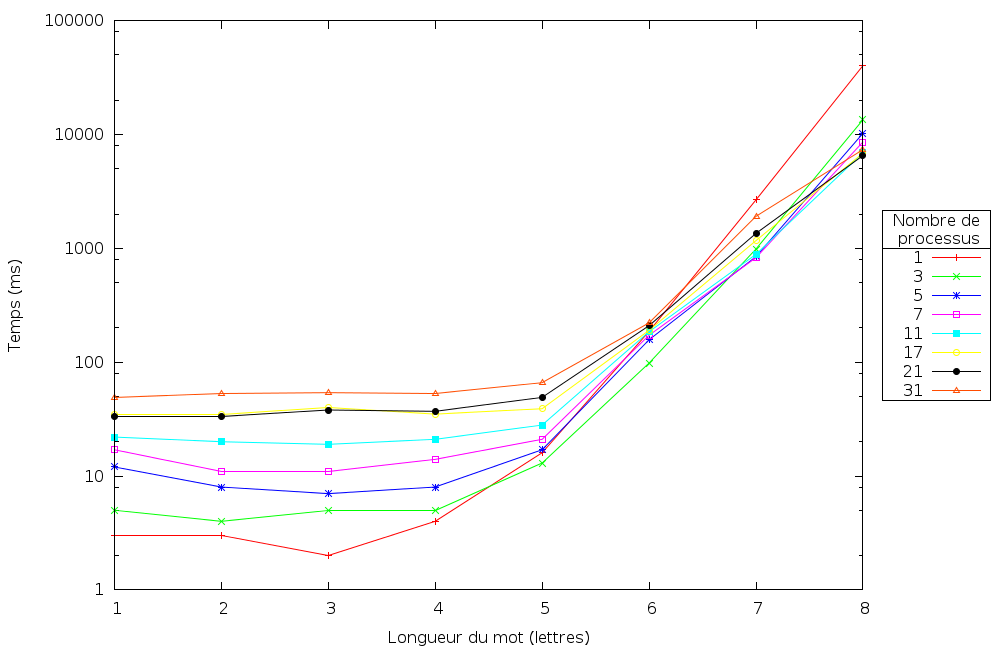
\includegraphics[width=\textwidth]{plot_log.png}
  \caption{Tests de performance, représentés sur une échelle logarithmique}
  \label{perf_loga}
\end{figure}

\begin{figure}[h!]
  \centering
  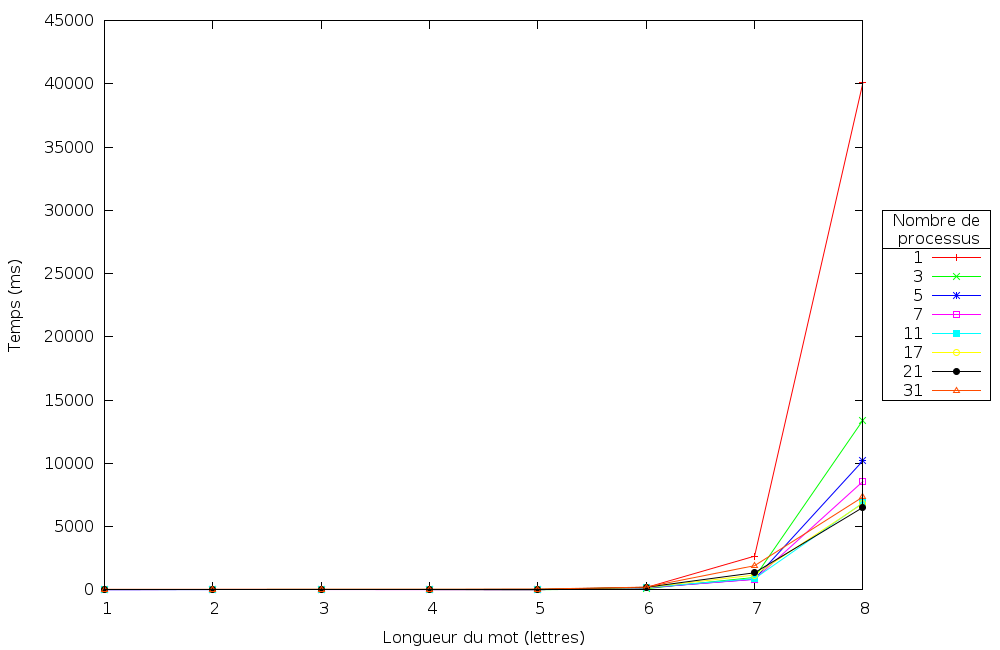
\includegraphics[width=\textwidth]{plot.png}
  \caption{Tests de performance}
  \label{perf}
\end{figure}

\section{Conclusion}

PVM permet de faire communiquer entre eux différents processus afin que les calculs s'effectuent sur plusieurs unités de calcul, et donc plus rapidement. Toutefois, l'archaïsme de la bibliothèque, avec par exemple la nécessité d'empaqueter les données avant chaque envoi et les multiples fonctions devant être appelées au préalable, ainsi que la difficulté supplémentaire lors de la recherche des bogues font qu'il est peu aisé de l'utiliser, notamment dans le cas où l'on souhaite multithreader les processus. En effet, PVM n'a pas été adapté pour un usage dans ce contexte, et par conséquent l'utilisateur doit prendre beaucoup de précautions. On peut toutefois remarquer le gain de performance appréciable apporté par la bibliothèque lorsque la taille de l'entrée devient importante. 


\end{document}
